\newpage
\section{Aufgabe 2: a}

\subsection{Aufgabenstellung}
Verwenden Sie als SMTP Ausgangsserver einen Ihrer eigenen Mailaccounts, z.B. den der
FH Bielefeld. Die Konfiguration kennen Sie aus den Hilfeseiten der DVZ. Das Programm
soll in der Lage sein, eine Mail mit einem von Ihnen vorgegebenen Inhalt an eine beliebige Mailadresse zu senden. Der Inhalt der Mail soll aus einer Datei inhalt.txt aus dem
Dateisystem Ihres Rechners eingelesen werden. (5 Punkte)


\subsection{Vorbereitung}
Zur Vorbereitung auf diese Aufgabe haben wir uns eine Entwicklungsumgebung unserer Wahl(IntelliJ) installiert und uns die Dokumentation zu Javamail angesehen.

\subsection{Durchführung}
Für diese Aufgabe stelle ich meinen FH Mailaccount zur Verfügung. Um eine Mail zu versenden brauchen wir zunächst einmal ein Session Objekt, welches ein Properties- und, auf Grund der TLS-Verschlüsselung, ein Authentificator-Objekt benötigt. 

\lstset{language=Java}
\begin{lstlisting}
from = "marti_niklas.stuwe@fh-bielefeld.de";
String user = "mstuwe@fh-bielefeld.de";
String password = "$$$";

Properties properties = System.getProperties();

properties.put("mail.smtp.host", "smtp.fh-bielefeld.de");
properties.put("mail.smtp.port", "587");
properties.put("mail.smtp.auth", "true");
properties.put("mail.smtp.starttls.enable", "true");

Authenticator auth = new Authenticator() {
	protected PasswordAuthentication getPasswordAuthentication() {
		return new PasswordAuthentication(user, password);
	}
};
this.session = Session.getDefaultInstance(properties, auth);
\end{lstlisting}

\begin{figure}[H]
	\centering
	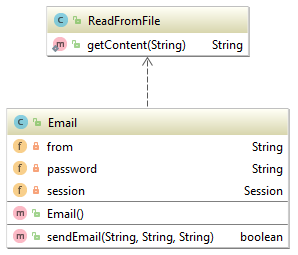
\includegraphics[width=0.4 \linewidth]{images/19}
	\caption{Klassendiagramm}
\end{figure}

\newpage
In diesem Teil des Codes wird die Nachricht aus Betreff, Empfänger, Inhalt und Absender zusammen gesetzt. Der Inhalt der E-Mail wird mit hilfe der statischen Methode \texttt{ReadFromFile.getContent()} aus der Datei gelesen.

\lstset{language=Java}
\begin{lstlisting}
MimeMessage msg = new MimeMessage(session);
msg.setSubject(subject);
msg.setFrom(from);

msg.setText(ReadFromFile.getContent(file));

msg.setRecipients(Message.RecipientType.TO, InternetAddress.parse(to, false));
Transport.send(msg);
\end{lstlisting}

\subsection{Fazit}
Bei dieser Aufgabe ist darauf zu achten, dass man sich am Mailserver der FH nicht mit der Mailadresse, sondern mit einem anderen Username anmeldet. Ansonsten gab es bei dieser Aufgabe keine Probleme.

\section{Aufgabe 2: b}
\subsection{Aufgabenstellung}
Erweitern Sie ihr Programm so, dass automatisch eine Liste von Empfängern aus der Datei
empfaenger.txt eingelesen wird. (1 Punkt)

\subsection{Vorbereitung}
Die Vorbereitung ist die vorherige Aufgabe. Die Mailadressen der Empfänger müssen unter einander in der Datei stehen(Eine pro Zeile).

\subsection{Durchführung}
Der Code muss nur minimal verändert werden, um das Versenden an mehrere Empfänger zu implementieren.

\lstset{language=Java}
\begin{lstlisting}
FileReader fr = new FileReader("res/empfaenger.txt");
BufferedReader br = new BufferedReader(fr);

String zeile = "";

while ((zeile = br.readLine()) != null) {
	msg.addRecipients(Message.RecipientType.TO, InternetAddress.parse(zeile, false));
	System.out.println(zeile);
}
br.close();
\end{lstlisting}

Das Hinzufügen der Empfänger wird nun durch eine Schleife realisiert, welche nach und nach alle Adressen aus der Datei als Recipients hinzufügt.

\subsection{Fazit}
Bei der Lösung dieser Aufgabe entstanden keine Probleme.

\section{Aufgabe 1: c}
\subsection{Aufgabenstellung}
Fugen Sie ihrer Mail einen Anhang hinzu (zum Beispiel ein Bild oder PDF-Dokument). Erläutern Sie, in welcher Form der Anhang übertragen wird.

\subsection{Vorbereitung}
Die Vorbereitung ist die vorherige Aufgabe.

\subsection{Durchführung}
Um einen Anhang zu versenden, muss man die Nachricht aus mehreren Teilen zusammensetzen. Da die Lösung so simpel wie möglich gelöst werden soll, senden wir den Anhang ohne Text direkt in der E-Mail.

\lstset{language=Java}
\begin{lstlisting}
MimeMessage msg = new MimeMessage(session);
msg.setSubject(subject);
msg.setFrom(from);

BodyPart messageBodyPart = new MimeBodyPart();
Multipart multipart = new MimeMultipart();

DataSource source = new FileDataSource(file);
messageBodyPart.setDataHandler(new DataHandler(source));
messageBodyPart.setFileName(file);
multipart.addBodyPart(messageBodyPart);

msg.setContent(multipart);
\end{lstlisting}

Wir benötigen ein Multipart Objekt, welches dann mit verschiedenen BodyParts gefüllt werden kann. Ein BodyPart ist in unserem Fall der besagte Anhang.

\subsection{Fazit}
Zum zweiten Teil der Aufgabe, sprich die Form der Übertragung von Anhängen, hat unsere Recherche kein Ergebnis ergeben.